% 作者:1FCENdoge、GaëlCHEN
% 日期:2022-05-06
%%
\documentclass{sysuthesis}
\usepackage{sysucode}  % 在论文中使用代码

%%
% 论文相关信息
% 本文档中前缀"c-"代表中文版字段, 前缀"e-"代表英文版字段
%%

% 扉页标题
% 论文题目应以简短、明确的词语恰当概括整个论文的核心内容,避免使用不常见的缩略词、缩写字。读者通过标题可大致了解毕业设计(论文)的内容、专业的特点和科学的范畴。中文题目一般不宜超过25个字。
\covertitlefirst{中山大学硕士毕业论文模板(试用)}
\covertitlesecond{\LaTeX\ template for undergraduate thesis of SYSU}
% 第二行英文标题,英文标题过长时使用,不用时留空即可,删除会导致编译问题
\covertitlethird{}

% 摘要页中文标题
\ctitle{中山大学硕士毕业论文模板(试用)}
% 摘要页英文标题
\etitle{\LaTeX\ template for undergraduate thesis of SYSU}


% 作者(扉页、摘要页)
\cauthor{小明}
\eauthor{Xiaoming}

% 专业(扉页、摘要页)
\cmajor{核技术及应用}
\emajor{Nuclear Technology and Application}

% 指导老师(扉页、摘要页)
\cmentor{大明(副教授)}
\ementor{Assoc. Prof. Daming}

     % 论文相关信息
%%
% 摘要
%%
% 中文摘要
\cabstract{

摘要内容应概括地反映出本论文的主要内容,主要说明本论文的研究目的、内容、方法、成果和结论。要突出本论文的创造性成果或新见解,不要与引言相混淆。语言力求精练、准确,硕士论文摘要以800-1200字为宜。在摘要的下方另起一行,注明本文的关键词(3-5个)。关键词是供检索用的主题词条,应采用能覆盖论文主要内容的通用技术词条(参照相应的技术术语标准)。按词条的外延层次排列,外延大的排在前面,每个关键词用“;”分开,最后一个关键词不打标点符号。}
% 中文关键词
\ckeywords{硕士学位论文;\LaTeX\ 模板;中山大学}

% 英文摘要
\eabstract{

The content of the abstract should generally reflect the main content of this paper, and mainly explain the research purpose, content, methods, results and conclusions of this paper. The creative achievements or new ideas of this paper should be highlighted, and should not be confused with the introduction. The language should be concise and accurate, and the length of abstract of the master's thesis should be properly. Start another line at the bottom of the summary, indicating the keywords of this article. Keywords are subject terms for retrieval, and general technical terms that can cover the main contents of the paper shall be adopted (refer to the corresponding technical terminology standards). According to the extension level of the entries, the ones with large extension are in the front, and each keyword is marked with ";" separate, the last keyword is not punctuated.
}
% 英文关键词
\ekeywords{Undergraduate thesis; \LaTeX\ template; Sun Yat-sen University}

     % 摘要内容
\begin{document}
% 论文前置部分
\frontmatter
\pagenumbering{Roman}
\maketitle    % 封面
% 定稿打印的论文需在扉页、学术诚信声明后添加空白页以保证这两部分内容各自独占一张纸,同时根据情况添加空白页以保证正文第一页为奇数页面,送盲审论文则可以不用添加空白页。
% 双数页面为空白页
\cleardoublepage
\makedisclaim    % 学术诚信声明
% 双数页面为空白页
\cleardoublepage
\makeabstract       % 中英文摘要
\maketableofcontents        % 目录
\newclearpage
\chapter{本文常用缩写对照表}

\newcommand{\tabincell}[2]{\begin{tabular}{@{}#1@{}}#2\end{tabular}}
% 上面一行的命令只需要在第一个需要拆分/合并单元格的表格中出现即可
\begin{table}[h]
	\renewcommand\arraystretch{1.5}
	\centering
	\begin{tabular}{|c|c|c|}
		\hline
		英文缩写 & 英文全称 & 中文翻译 \\
		\hline
		CFETR & \tabincell{c}{ China Fusion Engineering \\ Test Reactor } & 中国聚变工程试验堆 \\
		\hline
		ITER & \tabincell{c}{ International Thermonuclear \\ Experimental Reactor } & 国际热核聚变实验堆 \\
		\hline
		CPU & central processing unit & 中央处理器 \\
		\hline
		RISC & reduced instruction set computer & 精简指令集计算机 \\
		\hline
	\end{tabular}
\end{table}

% 双数页面为空白页
\cleardoublepage

% 论文主体部分
\mainmatter
% 正文
% 硕士学位论文一般有5到6章,博士学位论文一般有6到7章
%%
% 引言或背景
% 引言是论文正文的开端,应包括毕业论文选题的背景、目的和意义;对国内外研究现状和相关领域中已有的研究成果的简要评述;介绍本项研究工作研究设想、研究方法或实验设计、理论依据或实验基础;涉及范围和预期结果等。要求言简意赅,注意不要与摘要雷同或成为摘要的注解。
%%
% 章、节、小节、图片、公式、表格下方的\label{...}标记不建议删除,因为这些可以做到自动引用的作用,当某些公式、图片被删除时,\label{...}标记能使正文中的编号自动更新,省去一个一个编号的麻烦。

\chapter{绪论}
\label{cha:introduction}
\section{引言}
\label{sec:prologue}
引言是论文正文的开端,应包括毕业论文选题的背景、目的和意义;对国内外研究现状和相关领域中已有的研究成果的简要评述;介绍本项研究工作研究设想、研究方法或实验设计、理论依据或实验基础;涉及范围和预期结果等。要求言简意赅,注意不要与摘要雷同或成为摘要的注解。

\section{国内外研究现状和相关工作}
\label{sec:related_work}
对国内外研究现状和相关领域中已有的研究成果的简要评述。

\section{本文的论文结构与章节安排}
\label{sec:arrangement}
本文共分为五章,各章节内容安排如下:

第一章引言。

第二章知识点。

第三章方法介绍。

第四章实验和结果。

第五章是本文的最后一章,总结与展望。是对本文内容的整体性总结以及对未来工作的展望。


\newclearpage
\chapter{本模板的一些基本设定}
\label{cha:format}
本章将介绍本模板的一些基本设定。
\section{版面}
\label{sec:composition}
在介绍本模板的排版和格式之前,本章首先介绍一些基本的概念,如图 \ref{fig:composition_general} 所示。图 \ref{fig:composition_general} 中的英文为geometry宏包中的参数,纸张默认设置为A4大小,body或total body为正文内容所在区域。重要的参数有7个,分别是:top、bottom、left、right、headheight、headsep、footskip。top和bottom分别为上边距和下边距,本模板按照word默认设置为1英寸;left和right分别为左边距和右边距,本模板设置为1英寸;headsep为页眉(横线)与正文区域的距离,本模板按照word默认设置为0.2英寸;headheight为页眉内容的高度,本模板按照word默认设置页眉顶端距离页面边界1.5 cm,计算得到headheight为0.532 cm;footskip为页脚内容的高度,本模板按照word默认设置页脚底部距离页面边界1.75 cm,计算得到footskip为0.79 cm。
\begin{figure}[H] 
	\centering
	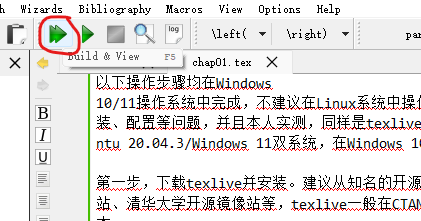
\includegraphics[width=0.6\textwidth]{image/chap01/f5.png}
	\caption{Build \& View}
	\label{fig:f5}
\end{figure}

每一章的标题采用小二号黑体,居中;节标题采用小三号宋体,加粗;小节标题采用小四号宋体,加粗(本模板中,由于选用的字库和字体问题,无法直接将宋体加粗,于是实际采用黑体代替宋体加粗)。正文内容、致谢和附录中的中文采用小四号宋体,英文采用Times New Roman,12 pt。参考文献的字体和字号采用宋体/Times New Roman,五号/10 pt。行距设置为1.5倍行距。



\newclearpage
\chapter{图像的插入示例}
\label{cha:fig_example}
除了第一章引言和最后一章的总结与展望之外,正文的所有章都要在章标题之下加上这样一段引入本章内容的话语,让读者知道本章的目的以及意义。本章将通过一些示例来说明如何插入图片。读者在阅读文章时,最能吸引读者注意力的莫过于文章中的图片,因此图片对于论文来说是重中之重,甚至可以说,好图就是好文章。规范地插入图片对于整篇文章的观感、阅读体验来说,有着至关重要的作用。
\section{单张图片的插入}
\label{sec:fig_singlefig}
单张图片插入的原则:(1)图片居中放置,大小适当,图中文字、内容清晰;(2)从文献中获得的图片要引用,要写明来源;(3)图片应该放置在两段文字之间,图片上面一段文字应该是对图片内容的描述,不要插在一段文字内,一页排不下时,应排在下一页的顶部;(4)对图片的描述要符合规范,指明是图x-x,不能说如下图所示。

错误描述:托卡马克装置示意图如下图所示\cite{xu2016general}:

正确描述:托卡马克装置示意图如图 \ref{fig:tokamak} 所示\cite{xu2016general}:
\begin{figure}[htbp] % 图片排序优先级,h表示当前位置,t表示顶部,b表示底部,p表示浮动页,可以是单独一个字母或者几个字母的组合
	% 居中
	\centering
	% 图片宽度、图片文件名及在硬盘中的位置
	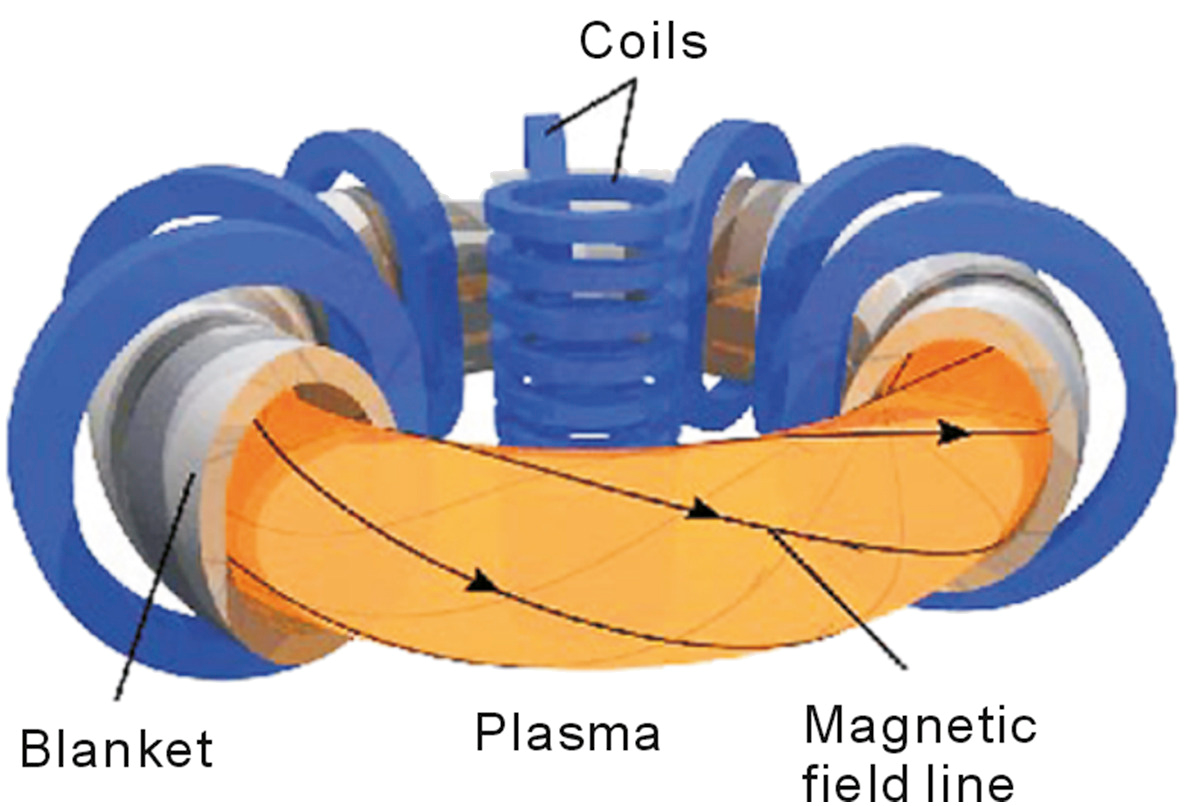
\includegraphics[width=0.6\textwidth]{image/chap03/tokamak.png}
	% 图片下标题
	\caption{托卡马克装置示意图\cite{xu2016general}}
	% 图片标签
	\label{fig:tokamak}
\end{figure}
\subsection{矢量图片的插入}
\label{ssec:fig_vecfig}
本小节示例了如何插入小节。按照中大的规定,正文中的标题只到小节,如 \ref{ssec:fig_vecfig} 小节,目录中的标题只到节,如 \ref{sec:fig_singlefig} 节。

\LaTeX\  支持svg、pdf、eps格式的矢量图的插入,svg格式的矢量图插入过程有点复杂,我暂时还没看明白,但是pdf和eps格式的矢量图是能直接插入的,操作很简单,与图 \ref{fig:tokamak} 操作相同,只需更改文件名。

图 \ref{fig:tbm_layer} 为插入的pdf格式的矢量图,图 \ref{fig:confusion} 为插入的eps格式的矢量图。一些简单的示意图可以用PowerPoint制作,最后导出成pdf即可,值得注意的是,MS Office套件由于自身的漏洞,无法导出eps格式的文件。
\begin{figure}[H] % H表示强制图片位置,配合float宏包使用,模板中已配置
	\centering
	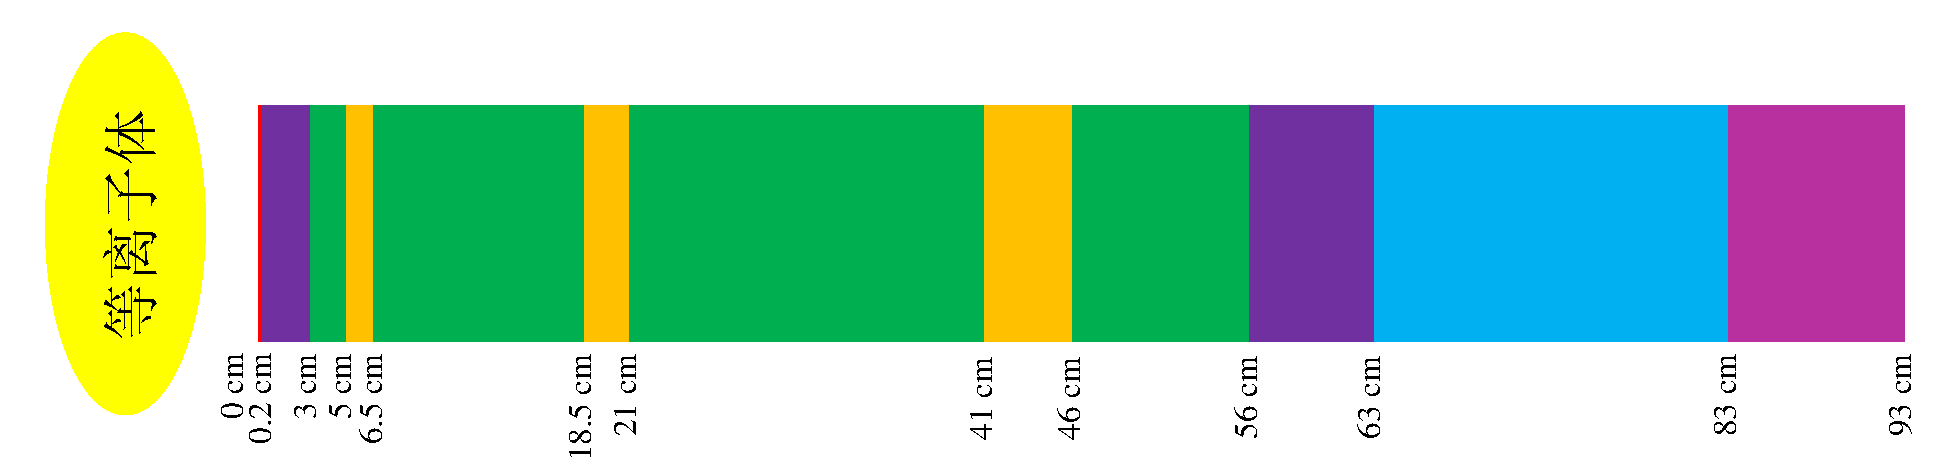
\includegraphics[width=1\textwidth]{image/chap03/tbm_layer.pdf}
	\caption{插入的pdf格式矢量图}
	\label{fig:tbm_layer}
\end{figure}
\begin{figure}[h]
	\centering
	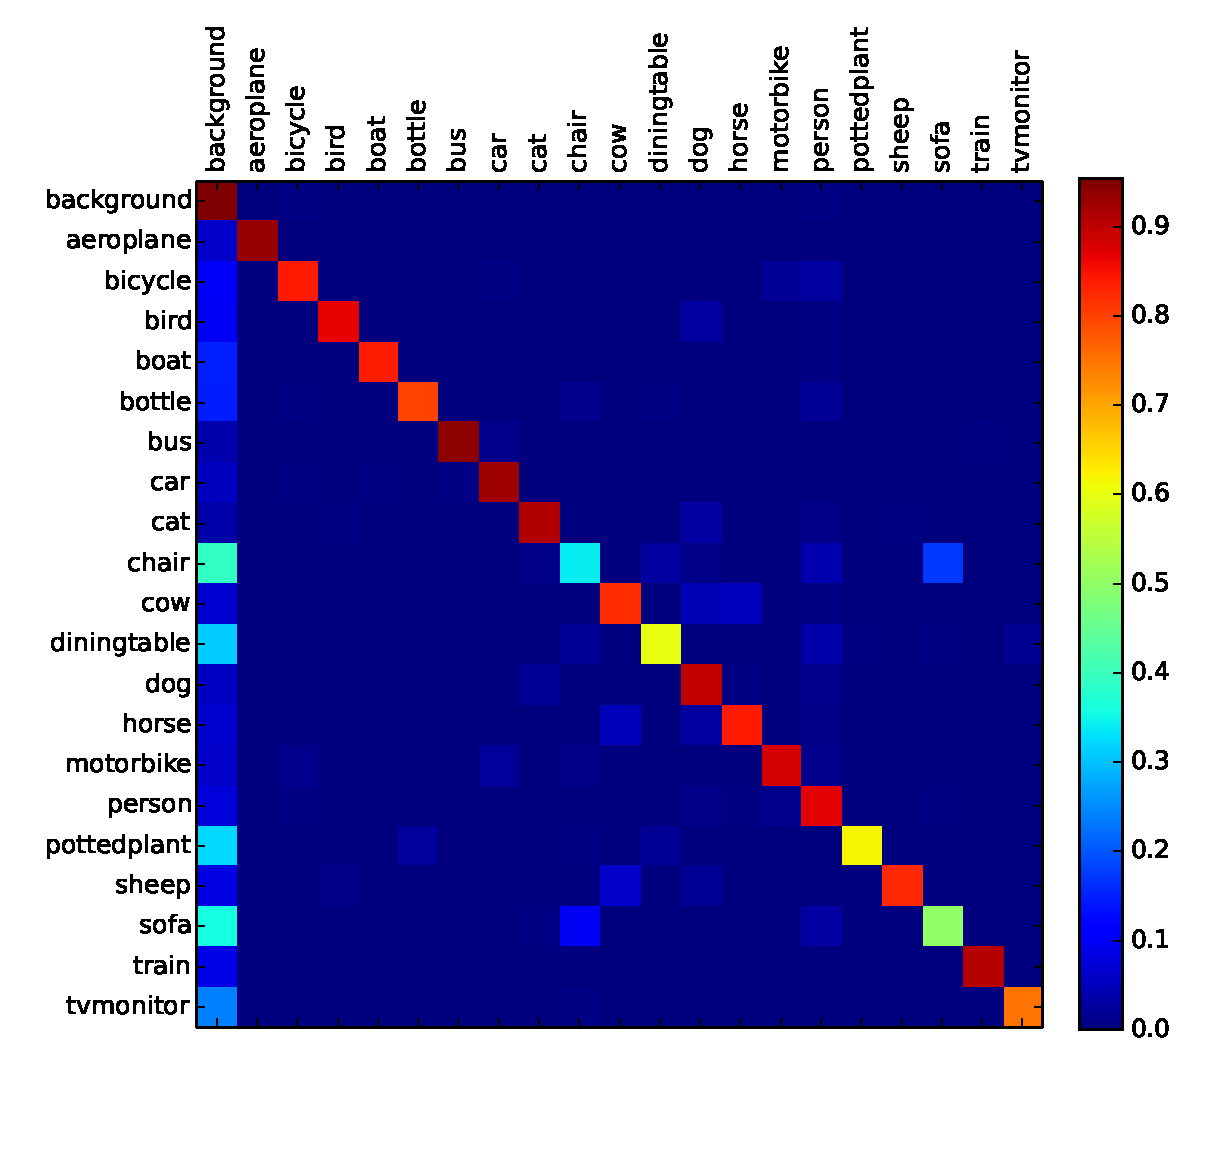
\includegraphics[width=0.6\textwidth]{image/chap03/confusion.eps}
	\caption{插入的eps格式矢量图}
	\label{fig:confusion}
\end{figure}
\section{多张图片的插入}
\label{sec:fig_multifig}
多张图片插入的原则与单张图片的相同,但是值得注意的是,多张图片不宜使用\LaTeX\ 直接插入,应将所需插入的图片先用PowerPoint排列、拼接,再标号,生成一张图片,再整个插入论文中,这样就与单张图片的插入过程相同。生成图片的过程,偷懒的话可以直接截屏保存为png格式图片,不偷懒就调整ppt的大小后直接导出为pdf。
\begin{figure}[h] 
	\centering
		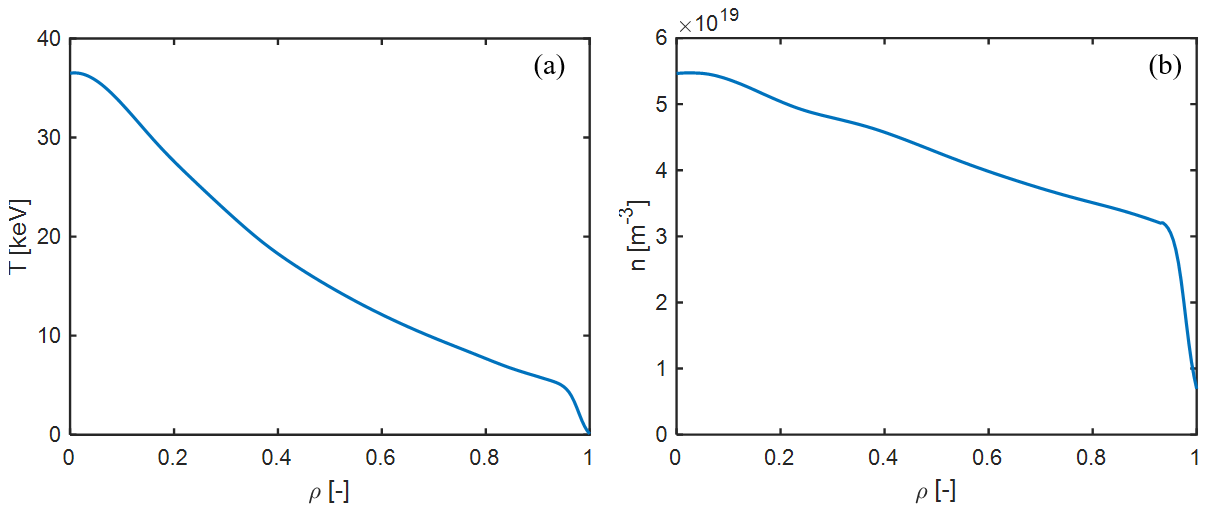
\includegraphics[width=1\textwidth]{image/chap03/temperature_density.png}
		\caption{简单的两张图片插入。(a)温度分布;(b)密度分布}
		\label{fig:temperature_density}
\end{figure}
\begin{figure}[h]
	\centering
	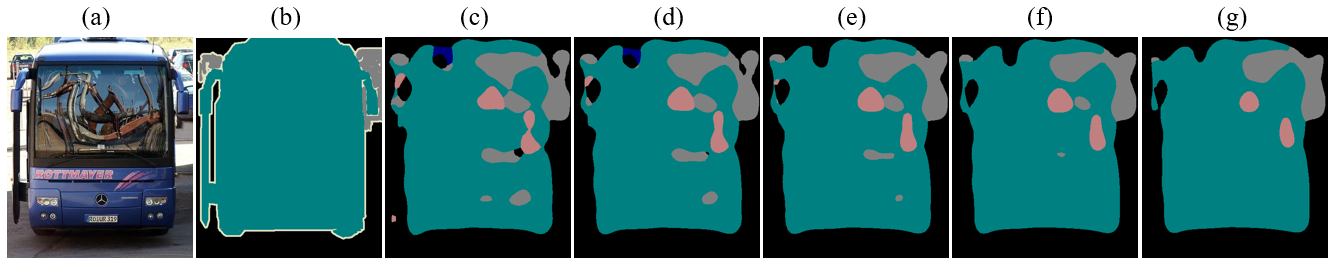
\includegraphics[width=1\textwidth]{image/chap03/compare.png}
	\caption{多张图片并排插入。(a)图像;(b)真值;(c) CNN+5LSTM1;(d) CNN+5LSTM2;\\ (e) CNN+5LSTM3;(f) CNN+5LSTM4;(g) CNN+5LSTM5}
	\label{fig:compare}
\end{figure}

\section{本章小结}

\newclearpage
\chapter{公式与表格的插入示例}
\label{cha:for_tab_example}
公式用于对论文基础理论的介绍,表格则是对一些不方便进行作图的数据进行展示。

\section{公式的插入}
\label{sec:formula}
带左半边大括号的核反应方程式,如式(\ref{eqn:fusion_reactions})所示:
\begin{equation}
	\label{eqn:fusion_reactions}
	\left\{
	\begin{aligned}
		&\mbox{D}+\mbox{D}\rightarrow \mbox{T}\,(\text{1.01}\;\mbox{MeV})+\mbox{p}\,(\text{3.03}\;\mbox{MeV}) \\
		&\mbox{D}+\mbox{D}\rightarrow {^{\text{3}}}\mbox{He}\,(\text{0.82}\;\mbox{MeV})+\mbox{n}\,(\text{2.45}\;\mbox{MeV}) \\
		&\mbox{D}+\mbox{T}\rightarrow \text{α}\,(\text{3.52}\;\mbox{MeV})+\mbox{n}\,(\text{14.06}\;\mbox{MeV}) \\
		&\mbox{D}+{^{\text{3}}}\mbox{He}\rightarrow \text{α}\,(\text{3.67}\;\mbox{MeV})+\mbox{p}\,(\text{14.67}\;\mbox{MeV})
	\end{aligned}
	\right.
\end{equation}

狄拉克函数$\delta_{ij}$的表达式:
\begin{equation}
	\label{eqn:delta_ij}
	\delta_{ij}=\left\{
	\begin{aligned}
		1&    &\mbox{if}&    &i=j \\
		0&    &\mbox{if}&    &i\neq j
	\end{aligned}
	\right.
\end{equation}

一般的公式:
\begin{equation}
	\label{eqn:vec_v_cm}
	\vec{v}_{cm}=\dfrac{m_{1}\vec{v}_{1}+m_{2}\vec{v}_{2}}{m_{1}+m_{2}}
\end{equation}

超长的公式:
\begin{equation}
	\label{eqn:iint_theta3_phi3}
	\begin{split}
		\int_{0}^{\pi}\int_{0}^{2\pi} \sin\theta_{3}&\dfrac{\exp(-\alpha v_{cm}^{2})}{v_{cm}}\sinh(\mu \gamma v_{r}v_{cm})\mbox{d}\phi_{3}\mbox{d}\theta_{3}=\dfrac{2\pi \sqrt{\pi}}{4\sqrt{\alpha}v_{3}u_{3}}\exp\left( \dfrac{(\mu \gamma v_{r})^{2}}{4\alpha} \right) \\
		&\times \Bigg( \mbox{erf}\left( \dfrac{\mu \gamma v_{r}+2\alpha(v_{3}-u_{3})}{2\sqrt{\alpha}} \right)-\mbox{erf}\left( \dfrac{-\mu \gamma v_{r}+2\alpha(v_{3}-u_{3})}{2\sqrt{\alpha}} \right) \\
		&+\mbox{erf}\left( \dfrac{-\mu \gamma v_{r}+2\alpha(v_{3}+u_{3})}{2\sqrt{\alpha}} \right)-\mbox{erf}\left( \dfrac{\mu \gamma v_{r}+2\alpha(v_{3}+u_{3})}{2\sqrt{\alpha}} \right) \Bigg)
	\end{split}
\end{equation}

输入矩阵:
\begin{equation}
	\label{eqn:matrix}
	\textbf{H} = \begin{bmatrix}
		I*\mybold{x}_i \\ \textbf{h}
	\end{bmatrix}
\end{equation}
\newclearpage
\chapter{结论与展望}
\label{cha:conclusion_outlook}
\newclearpage
%% 第六章,有需要可自行使用
%\newclearpage
%\include{docs/chap07}
%\newclearpage

% 附录部分
\backmatter
% 参考文献。因不需要纳入章节目录,故放入附录部分
% 实际上参考文献是属于论文主体部分
\makereferences
% 每一个引用之间不添加多余间距
\setlength{\bibsep}{0em}
% 引用样式
\bibliographystyle{bibtex-style/gbt7714-2015-numerical}
{\zihao{5}\rmfamily\songti\bibliography{reference}}    % 引用文献列表
\newclearpage
% 论文送盲审时使用
%\begin{publications}{99}
%
%\begin{table}[h]
%	\renewcommand\arraystretch{1.5}
%	\centering
%	\begin{tabular}{|*{6}{c|}}
%		\hline
%		\tabincell{c}{ 序 \\ 号 } & 发表或投稿刊物/会议名称 & \tabincell{c}{ 作者(仅注\\明第几作\\者) } & \tabincell{c}{发表\\年份} & \tabincell{c}{与学位论\\文哪一部\\分(章、节)\\相关} & \tabincell{c}{被索引\\收录情\\况} \\
%		\hline
%		1 & \tabincell{c}{ 2008 19th International\\ Conference on Pattern\\ Recognition } & 第一作者 & 2008 & 第二章 & EI收录 \\
%		\hline
%		2 & \tabincell{c}{ Asian Conference \\ on Computer Vision } & 第一作者 & 2009 & 第三章 & EI收录 \\
%		\hline
%		3 & \tabincell{c}{ 2010 20th International\\ Conference on Pattern\\ Recognition } & 第一作者 & 2010 & 第三章 & EI收录 \\
%		\hline
%		4 & \tabincell{c}{ International journal of\\ innovative computing,\\ information \& control } & 第一作者 & 2011 & 第四章 & SCI收录 \\
%		\hline
%		5 & \tabincell{c}{ Journal of Industrial\\ and Management\\ Optimization (JIMO) } & 第一作者 & 2012 & 第四章 & SCI收录 \\
%		\hline
%	\end{tabular}
%\end{table}
%
%\end{publications}

% 论文定稿打印时使用
\begin{publications}{99}
\setlength{\itemsep}{0em}

\item \textbf{Qiu H}, Lai J, Huang J, et al. Semi-supervised discriminant analysis based on UDP regularization[C]. 2008 19th International Conference on Pattern Recognition. IEEE, 2008: 1-4.

\item \textbf{Qiu H}, Liu W, Lai J H. Gender recognition via locality preserving tensor analysis on face images[C]. Asian Conference on Computer Vision. Springer, Berlin, Heidelberg, 2009: 601-610.

\item \textbf{Qiu H}, Pham D S, Venkatesh S, et al. A fast extension for sparse representation on robust face recognition[C]. 2010 20th International Conference on Pattern Recognition. IEEE, 2010: 1023-1027.

\item \textbf{Qiu H}, Pham D S, Venkatesh S, et al. Innovative sparse representation algorithms for robust face recognition[J]. International journal of innovative computing, information \& control, 2011, 7(10): 5645-5667.

\item \textbf{Qiu H}, Chen X, Liu W, et al. A fast $\ell_1$-solver and its applications to robust face recognition[J]. Journal of Industrial and Management Optimization (JIMO), 2012, 8: 163-178.

\end{publications}
% 致谢
% 送盲审论文暂时不需要致谢,将下面一行代码注释掉即可,待论文答辩、定稿打印时再添加致谢
%%
% 致谢
% 谢辞应以简短的文字对课题研究与论文撰写过程中曾直接给予帮助的人员(例如指导教师、答疑教师及其他人员)表示对自己的谢意,这不仅是一种礼貌,也是对他人劳动的尊重,是治学者应当遵循的学术规范。内容限一页。
% modifier: 黄俊杰
% update date: 2017-04-15
%%

\chapter{致谢}

	

%\vskip 108pt
%\begin{flushright}
%	黄汉宇\makebox[1cm]{} \\
%\today
%\end{flushright}


\newclearpage
% 附录
\appendix
\chapter{补充更多细节}

\begin{figure}[h!]
\centering
		\makebox[0.16\textwidth]{\scriptsize 图像}
		\makebox[0.16\textwidth]{\scriptsize 真值}
		\makebox[0.16\textwidth]{\scriptsize Grid-5LSTM1}
		\makebox[0.16\textwidth]{\scriptsize Grid-5LSTM3}
		\makebox[0.16\textwidth]{\scriptsize Grid-5LSTM5} \\
		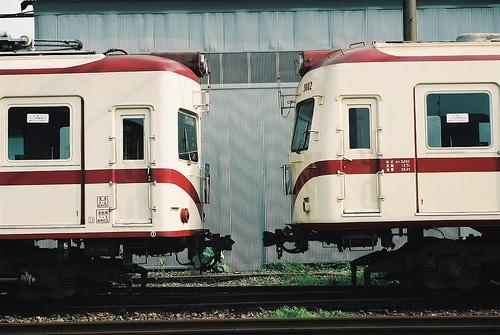
\includegraphics[width=0.16\textwidth]{image/appendix1/2007_000042.jpg}
		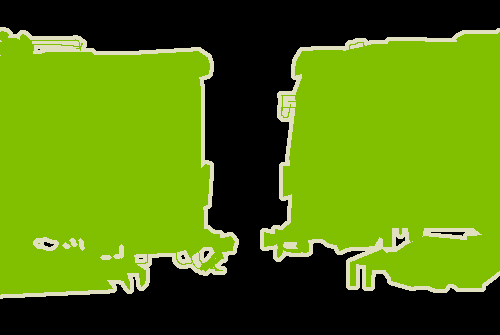
\includegraphics[width=0.16\textwidth]{image/appendix1/2007_000042.png}
		
\includegraphics[width=0.16\textwidth]{image/appendix1/1/2007_000042.png} 
		
\includegraphics[width=0.16\textwidth]{image/appendix1/3/2007_000042.png}
		
\includegraphics[width=0.16\textwidth]{image/appendix1/5/2007_000042.png} \\

		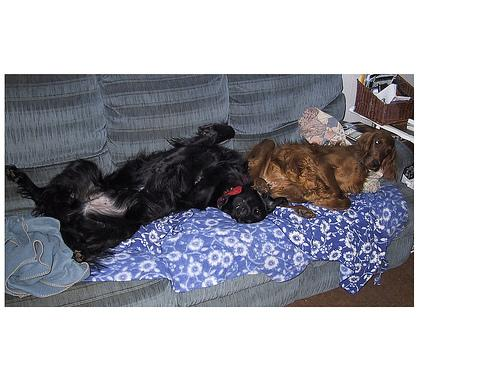
\includegraphics[width=0.16\textwidth]{image/appendix1/2011_003256.jpg}
		
\includegraphics[width=0.16\textwidth]{image/appendix1/2011_003256.png}
		
\includegraphics[width=0.16\textwidth]{image/appendix1/1/2011_003256.png} 
		
\includegraphics[width=0.16\textwidth]{image/appendix1/3/2011_003256.png}
		
\includegraphics[width=0.16\textwidth]{image/appendix1/5/2011_003256.png} \\
		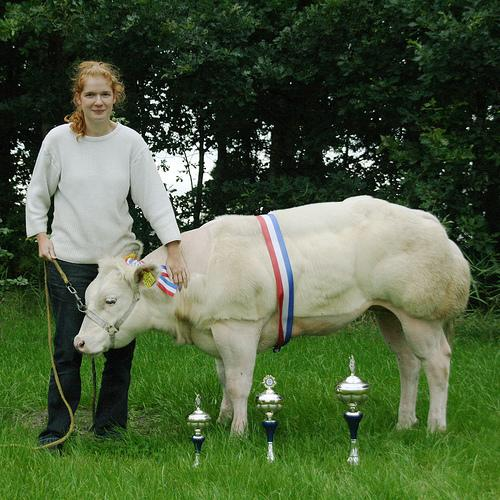
\includegraphics[width=0.16\textwidth]{image/appendix1/2011_001159.jpg}
		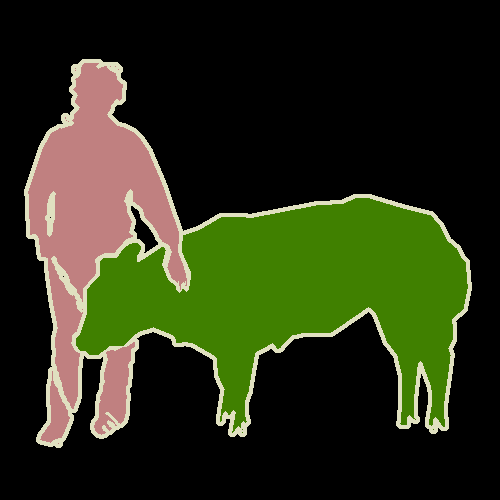
\includegraphics[width=0.16\textwidth]{image/appendix1/2011_001159.png}
		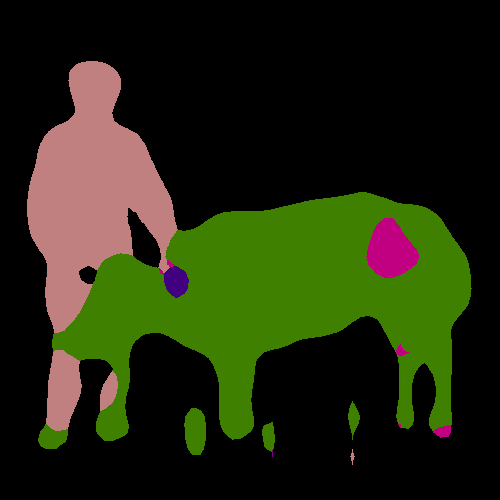
\includegraphics[width=0.16\textwidth]{image/appendix1/1/2011_001159.png} 
		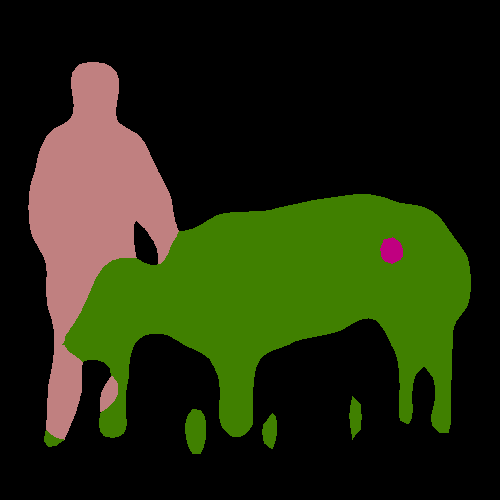
\includegraphics[width=0.16\textwidth]{image/appendix1/3/2011_001159.png}
		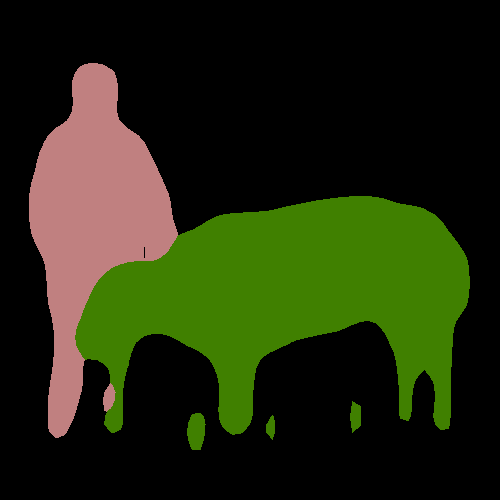
\includegraphics[width=0.16\textwidth]{image/appendix1/5/2011_001159.png} \\
		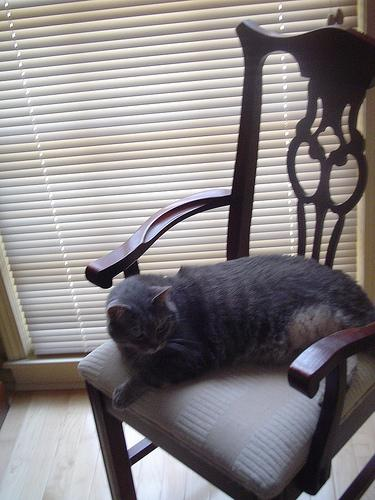
\includegraphics[width=0.16\textwidth]{image/appendix1/2011_000813.jpg}
		
\includegraphics[width=0.16\textwidth]{image/appendix1/2011_000813.png}
		
\includegraphics[width=0.16\textwidth]{image/appendix1/1/2011_000813.png} 
		
\includegraphics[width=0.16\textwidth]{image/appendix1/3/2011_000813.png}
		
\includegraphics[width=0.16\textwidth]{image/appendix1/5/2011_000813.png} \\
		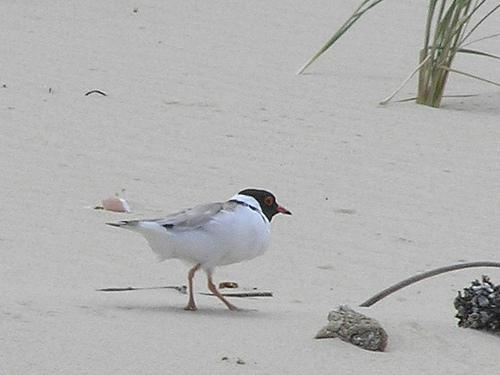
\includegraphics[width=0.16\textwidth]{image/appendix1/2011_003145.jpg}
		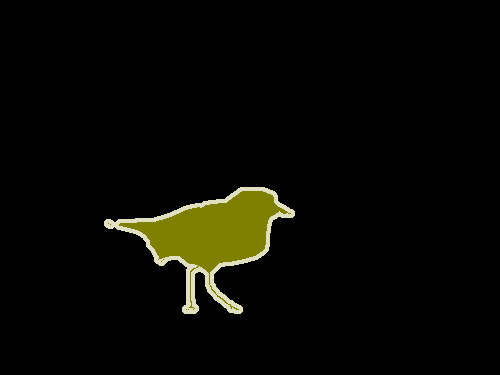
\includegraphics[width=0.16\textwidth]{image/appendix1/2011_003145.png}
		
\includegraphics[width=0.16\textwidth]{image/appendix1/1/2011_003145.png} 
		
\includegraphics[width=0.16\textwidth]{image/appendix1/3/2011_003145.png}
		
\includegraphics[width=0.16\textwidth]{image/appendix1/5/2011_003145.png} \\
		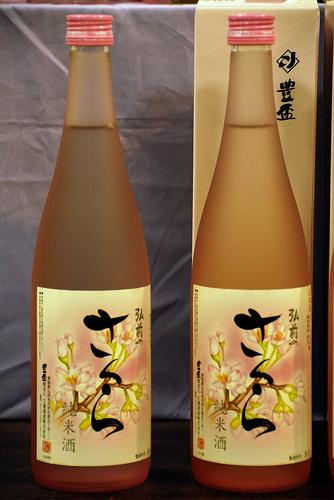
\includegraphics[width=0.16\textwidth]{image/appendix1/2009_004579.jpg}
		
\includegraphics[width=0.16\textwidth]{image/appendix1/2009_004579.png}
		
\includegraphics[width=0.16\textwidth]{image/appendix1/1/2009_004579.png} 
		
\includegraphics[width=0.16\textwidth]{image/appendix1/3/2009_004579.png}
		
\includegraphics[width=0.16\textwidth]{image/appendix1/5/2009_004579.png} \\
\color[rgb]{0.9,0.9,0.9}\bfseries
\begin{tabular}{*{7}{>{\centering\arraybackslash}p{0.10\textwidth}}}
	\hline
	\cellcolor[rgb]{0,0,0}  背景&\cellcolor[rgb]{0.5020,0,0} 飞机 &\cellcolor[rgb]{0,0.5020,0} 自行车 &\cellcolor[rgb]{0.5020,0.5020,0} 鸟 &\cellcolor[rgb]{0,0,0.5020} 船   &\cellcolor[rgb]{0.5020,0,0.5020} 瓶子 &\cellcolor[rgb]{0,0.5020,0.5020} 大巴
	\\
	\hline
	\cellcolor[rgb]{0.5020,0.5020,0.5020} 汽车 & \cellcolor[rgb]{0.2510,0,0} 猫 &\cellcolor[rgb]{0.7529,0,0} 椅子 &\cellcolor[rgb]{0.2510,0.5020,0} 牛 &\cellcolor[rgb]{0.7529,0.5020,0} 桌子 &\cellcolor[rgb]{0.2510,0,0.5020} 狗 &\cellcolor[rgb]{0.7529,0,0.5020} 马 \\
	\hline
	\cellcolor[rgb]{0.2510,0.5020,0.5020} 摩托车 &\cellcolor[rgb]{0.7529,0.5020,0.5020} 人   &\cellcolor[rgb]{0,0.2510,0} 盆栽   &\cellcolor[rgb]{0.5020,0.2510,0} 羊 &\cellcolor[rgb]{0,0.7529,0} 沙发 &\cellcolor[rgb]{0.5020,0.7529,0} 火车 &\cellcolor[rgb]{0,0.2510,0.5020} 电视 \\
	\hline
\end{tabular}

\caption{一个配有彩色表格的插图}
\end{figure}

\endinput

\chapter{MCNP输入卡}

\begin{python}
1D model of CFETR core                                                          
c cell card for CFETR core                                                     
1 0 -1 25 -26
2 6 -5.75 1 -2 25 -26
3 0 2 -3 25 -26
4 4 -8.017 3 -4 25 -26
5 0 4 -5 25 -26
6 3 -7.709 5 -6 25 -26
7 0 6 -7 25 -26
8 2 -4.515 7 -8 25 -26
9 1 -3.433 8 -9 25 -26
10 0 9 -10 25 -26
11 0 10 -11 25 -26
12 0 11 -12 25 -26
13 1 -3.433 12 -13 25 -26
14 0 13 -14 25 -26
15 2 -4.515 14 -15 25 -26
16 0 15 -16 25 -26
17 3 -7.709 16 -17 25 -26
18 0 17 -18 25 -26
19 4 -8.017 18 -19 25 -26
20 0 19 -20 25 -26
21 3 -7.709 20 -21 25 -26
22 0 21 -22 25 -26
23 5 -7.93 22 -23 25 -26
24 0 23 -24 25 -26
25 0 24:-25:26                                          

c surface card
1 CZ 115
2 CZ 225
3 CZ 240.5
4 CZ 348                                            
5 CZ 353
6 CZ 357
7 CZ 362
8 CZ 392
9 CZ 486
10 CZ 500                                                                    
11 CZ 940                                                                     
12 CZ 968                                                                     
13 CZ 1088                                                                    
14 CZ 1238                                                                    
15 CZ 1276                                                                    
16 CZ 1291                                                                  
17 CZ 1295                                                                 
18 CZ 1312                                                                 
19 CZ 1401.5
20 CZ 1418.5
21 CZ 1422.5                                                               
22 CZ 1430
23 CZ 1435
24 CZ 2113
*25 PZ -1000
*26 PZ 1000

mode n
c importance card
imp:n 16 16 8 8 4 4 2 2 2 1 1 1 2 2 4 4 8 8 16 32 64 64 150 150 0
c -----------material of BLK   rho=3.433 g/cm3
c CLF-1 volum%  0.3572
M1 26054.21c 1.84904E+00  $  Fe540.058   5.8%
26056.21c 2.92339E+01  $  Fe560.917  91.7%
26057.21c 7.01359E-01  $  Fe570.022   2.2%
26058.21c 9.56399E-02  $  Fe580.003   0.3%
8016.21c  1.24782E-02  $  O16
24050.21c 1.48592E-01  $  Cr500.043   4.3%
24052.21c 2.89582E+00  $  Cr520.838  83.8%
24053.21c 3.31741E-01  $  Cr530.096   9.6%
24054.21c 8.29354E-02  $  Cr540.024   2.4%
42092.21c 1.54405E-04  $  Mo         (nat.)
42094.21c 9.62429E-05
42095.21c 1.65642E-04
42096.21c 1.73549E-04
42097 9.93641E-05
42098.21c 2.51064E-04
42100 1.00197E-04
25055.21c 1.45359E-01  $  Mn55
28058.21c 1.15268E-03  $  Ni58.678   67.8%
28060.21c 4.45432E-04  $  Ni60.262   26.2%
28061.21c 2.21016E-05  $  Ni61.013    1.3%
28062.21c 6.29043E-05  $  Ni62.037    3.7%
28064.21c 2.04014E-05  $  Ni64.012    1.2%
74182.21c 3.15349E-02  $  W1820.264  26.4%
74183.21c 1.72009E-02  $  W1830.144  14.4%
74184.21c 3.65519E-02  $  W1840.306  30.6%
74186.21c 3.39240E-02  $  W1860.284  28.4%
23000.21c 7.83815E-02  $  V         (nat.)
29063.21c 1.08667E-03  $  Cu630.691  69.1%
29065.21c 4.85938E-04  $  Cu650.309  30.9%
41093.21c 2.14887E-04  $  Nb93
27059.21c 1.69209E-03  $  Co59
13027.21c 7.39926E-03  $  Al27
73181.21c 7.72324E-03  $  Ta181
22046.21c 3.43853E-04  $  Ti         (nat.)
22047.21c 3.10093E-04
22048.21c 3.07259E-03
22049.21c 2.25484E-04
22050.21c 2.15898E-04
c Li4SiO4 volum% 0.0462  
14028.21c 1.08478E-02
14029.21c 5.50824E-04
14030.21c 3.63107E-04
3006.21c 3.92335E-02
3007.21c 4.35928E-03
22046.21c 5.33766E-08
22047.21c 4.81360E-08
22048.21c 4.76961E-07
22049.21c 3.50021E-08
22050.21c 3.35141E-08
29063.21c 7.03133E-07
29065.21c 3.13396E-07
40000.21c 4.24004E-08
11023.21c 1.39697E-05
82206.21c 2.35718E-08
82207.21c 2.16157E-08
82208.21c 5.12516E-08
30000.42c 9.46276E-08
13027.21c 8.55398E-07
26054.21c 5.52069E-08
26056.21c 8.66630E-07
26057.21c 2.00143E-08
26058.21c 2.66353E-09
20000 6.77600E-06
8016.21c 4.52716E-02
c Be volum% 0.186 
26054.21c 7.58603E-07
26056.21c 1.19938E-05
26057.21c 2.87746E-07
26058.21c 3.92382E-08
82206.21c 3.9062E-08 
82207.21c 3.58203E-08
82208.21c 8.49315E-08
8016.21c 5.37358E-05
4009.21c 0.185724906
6012.21c 0.000113241
20000 8.37913E-07
12000.21c 1.7272E-05 
14028.21c 6.37195E-06
14029.21c 3.23553E-07
14030.21c 2.13288E-07
42092.21c 5.19472E-08
42094.21c 3.23794E-08
42095.21c 5.57276E-08
42096.21c 5.8388E-08 
42097 3.34296E-08
42098.21c 8.44667E-08
42100 3.37097E-08
24050.21c 8.33196E-09
24052.21c 1.62377E-06
24053.21c 1.86017E-07
24054.21c 4.65039E-08
7014.21c 4.55559E-05
13027.21c 1.55587E-05
27059.21c 1.13972E-07
29063.21c 7.30377E-07
29065.21c 3.26609E-07
40000.21c 1.8408E-07 
47107.66c 2.42094E-08
47109.66c 2.24917E-08
21045.66c 1.86759E-07
22046.21c 1.15685E-07
22047.21c 1.04326E-07
22048.21c 1.03373E-06
22049.21c 7.5861E-08 
22050.21c 7.2636E-08 
74182.21c 2.41121E-07
74183.21c 1.31521E-07
74184.21c 2.79482E-07
74186.21c 2.5939E-07
c Water volum% 0.1438
1001.21c 0.095933404
1002.21c 1.10336E-05
8016.21c 0.047855621
c material of VV rho=4.515 g/cm3
c 316SS-LN volum% 0.5
M2 6012.21c 6.92225E-04 $ C 12 weight(%)  0.0300 ab(%) 98.93
25055.21c 1.00801E-02 $Mn 55 weight(%)  2.0000
28058.21c 3.85387E-02 $Ni 58 weight(%) 12.0000 ab(%) 68.08
28060.21c 1.48450E-02 $Ni 60 weight(%) 12.0000 ab(%) 26.22
28061.21c 6.45305E-04 $Ni 61 weight(%) 12.0000 ab(%)  1.14
28062.21c 2.05751E-03 $Ni 62 weight(%) 12.0000 ab(%)  3.63
28064.21c 5.23988E-04 $Ni 64 weight(%) 12.0000 ab(%)  0.93
24050.21c 3.93347E-03 $Cr 50 weight(%) 17.0000 ab(%)  4.35
24052.21c 7.58531E-02 $Cr 52 weight(%) 17.0000 ab(%) 83.79
24053.21c 8.60114E-03 $Cr 53 weight(%) 17.0000 ab(%)  9.50
24054.21c 2.14101E-03 $Cr 54 weight(%) 17.0000 ab(%)  2.37
42092.21c 1.07083E-03 $Mo 92 weight(%)  2.5000 ab(%) 14.84
42094.21c 6.67465E-04 $Mo 94 weight(%)  2.5000 ab(%)  9.25
42095.21c 1.14876E-03 $Mo 95 weight(%)  2.5000 ab(%) 15.92
42096.21c 1.20360E-03 $Mo 96 weight(%)  2.5000 ab(%) 16.68
42097 6.89113E-04 $Mo 97 weight(%)  2.5000 ab(%)  9.55
42098.21c 1.74118E-03 $Mo 98 weight(%)  2.5000 ab(%) 24.13
42100 6.94885E-04 $Mo100 weight(%)  2.5000 ab(%)  9.63
7014.21c 2.75749E-03 $ N 14 weight(%)  0.1400 ab(%) 99.63
7015.21c 1.01850E-05 $ N 15 weight(%)  0.1400 ab(%)  0.37
15031.21c 4.02273E-04 $ P 31 weight(%)  0.0450
16000.21c 2.59064E-04 $ S  0 weight(%)  0.0300
14028.21c 6.81875E-03 $Si 28 weight(%)  0.7500 ab(%) 92.22
14029.21c 3.46779E-04 $Si 29 weight(%)  0.7500 ab(%)  4.69
14030.21c 2.28475E-04 $Si 30 weight(%)  0.7500 ab(%)  3.09
41093.21c 2.98032E-05 $Nb 93 weight(%)  0.0100
73181.21c 1.53021E-05 $Ta181 weight(%)  0.0100 ab(%) 99.99
22046.21c 7.15622E-05 $Ti 46 weight(%)  0.1500 ab(%)  8.25
22047.21c 6.45361E-05 $Ti 47 weight(%)  0.1500 ab(%)  7.44
22048.21c 6.39462E-04 $Ti 48 weight(%)  0.1500 ab(%) 73.72
22049.21c 4.69275E-05 $Ti 49 weight(%)  0.1500 ab(%)  5.41
22050.21c 4.49324E-05 $Ti 50 weight(%)  0.1500 ab(%)  5.18
29063.21c 9.04191E-04 $Cu 63 weight(%)  0.3000 ab(%) 69.17
29065.21c 4.03010E-04 $Cu 65 weight(%)  0.3000 ab(%) 30.83
27059.21c 2.34919E-04 $Co 59 weight(%)  0.0500
5010.21c 5.09675E-06 $ B 10 weight(%)  0.0010 ab(%) 19.90
5011.21c 2.05150E-05 $ B 11 weight(%)  0.0010 ab(%) 80.10
13027.21c 5.13109E-04 $Al 27 weight(%)  0.0500
8016.21c 3.46222E-05 $ O 16 weight(%)  0.0020 ab(%) 99.76
19000 3.54062E-06 $ K  0 weight(%)  0.0005
83209.21c 1.05997E-06 $Bi209 weight(%)  0.0008
23000.21c 2.17407E-05 $ V  0 weight(%)  0.0040
40000.21c 6.06990E-06 $Zr  0 weight(%)  0.0020
50000.21c 4.66499E-06 $Sn  0 weight(%)  0.0020
74182.21c 3.99560E-07 $ W182 weight(%)  0.0010 ab(%) 26.50
74183.21c 2.15838E-07 $ W183 weight(%)  0.0010 ab(%) 14.31
74184.21c 4.62047E-07 $ W184 weight(%)  0.0010 ab(%) 30.64
74186.21c 4.28631E-07 $ W186 weight(%)  0.0010 ab(%) 28.43
82206.21c 2.61226E-07 $Pb206 weight(%)  0.0008 ab(%) 24.10
82207.21c 2.39548E-07 $Pb207 weight(%)  0.0008 ab(%) 22.10
82208.21c 5.67978E-07 $Pb208 weight(%)  0.0008 ab(%) 52.40
26054.21c 1.88145E-02 $Fe 54 weight(%) 64.9209 ab(%)  5.85
26056.21c 2.95347E-01 $Fe 56 weight(%) 64.9209 ab(%) 91.75
26057.21c 6.82083E-03 $Fe 57 weight(%) 64.9209 ab(%)  2.12 
c    water volum% 0.5
1001.21c 0.333565246
1002.21c 3.83644E-05
8016.21c 0.16639639
c material of TS rho=7.709 g/cm3
M3 6012.21c 3.09498E-004 $ C 12 weight(%)  0.0800
25055.21c 1.69007E-003 $Mn 55 weight(%)  2.0000
15031.21c 6.74470E-005 $ P 31 weight(%)  0.0450
16000.21c 4.34359E-005 $ S  0 weight(%)  0.0300
14028.21c 1.14326E-003 $Si 28 weight(%)  0.7500 ab(%) 92.22
14029.21c 5.81426E-005 $Si 29 weight(%)  0.7500 ab(%)  4.69
14030.21c 3.83072E-005 $Si 30 weight(%)  0.7500 ab(%)  3.09
24050.21c 7.37094E-004 $Cr 50 weight(%) 19.0000 ab(%)  4.35
24052.21c 1.42141E-002 $Cr 52 weight(%) 19.0000 ab(%) 83.79
24053.21c 1.61177E-003 $Cr 53 weight(%) 19.0000 ab(%)  9.50
24054.21c 4.01203E-004 $Cr 54 weight(%) 19.0000 ab(%)  2.37
28058.21c 7.26928E-003 $Ni 58 weight(%) 13.5000 ab(%) 68.08
28060.21c 2.80011E-003 $Ni 60 weight(%) 13.5000 ab(%) 26.22
28061.21c 1.21719E-004 $Ni 61 weight(%) 13.5000 ab(%)  1.14
28062.21c 3.88094E-004 $Ni 62 weight(%) 13.5000 ab(%)  3.63
28064.21c 9.88360E-005 $Ni 64 weight(%) 13.5000 ab(%)  0.93
7014.21c 3.30238E-004 $ N 14 weight(%)  0.1000 ab(%) 99.63
7015.21c 1.21976E-006 $ N 15 weight(%)  0.1000 ab(%)  0.37
5010.21c 5.28557E-003 $ B 10 weight(%)  1.1400
5011.21c 2.53012E-004 $ B 11 weight(%)  0.0600
27059.21c 3.93875E-005 $Co 59 weight(%)  0.0500
41093.21c 4.99693E-006 $Nb 93 weight(%)  0.0100
73181.21c 2.56563E-006 $Ta181 weight(%)  0.0100
22046.21c 1.19985E-005 $Ti 46 weight(%)  0.1500 ab(%)  8.25
22047.21c 1.08204E-005 $Ti 47 weight(%)  0.1500 ab(%)  7.44
22048.21c 1.07215E-004 $Ti 48 weight(%)  0.1500 ab(%) 73.72
22049.21c 7.86808E-006 $Ti 49 weight(%)  0.1500 ab(%)  5.41
22050.21c 7.53358E-006 $Ti 50 weight(%)  0.1500 ab(%)  5.18
29063.21c 5.05337E-005 $Cu 63 weight(%)  0.1000 ab(%) 69.17
29065.21c 2.25235E-005 $Cu 65 weight(%)  0.1000 ab(%) 30.83
13027.21c 8.60303E-005 $Al 27 weight(%)  0.0500
8016.21c 5.80493E-006 $ O 16 weight(%)  0.0020
19000 5.93637E-007 $ K  0 weight(%)  0.0005
83209.21c 1.77719E-007 $Bi209 weight(%)  0.0008
23000.21c 3.64516E-006 $ V  0 weight(%)  0.0040
40000.21c 1.01771E-006 $Zr  0 weight(%)  0.0020
50000.21c 7.82154E-007 $Sn  0 weight(%)  0.0020
c    56138.10c 1.68328E-007 $Ba138 weight(%)  0.0005
74182.21c 6.69920E-008 $ W182 weight(%)  0.0010 ab(%) 26.50
74183.21c 3.61885E-008 $ W183 weight(%)  0.0010 ab(%) 14.31
74184.21c 7.74688E-008 $ W184 weight(%)  0.0010 ab(%) 30.64
74186.21c 7.18664E-008 $ W186 weight(%)  0.0010 ab(%) 28.43
82206.21c 4.37984E-008 $Pb206 weight(%)  0.0008 ab(%) 24.10
82207.21c 4.01637E-008 $Pb207 weight(%)  0.0008 ab(%) 22.10
82208.21c 9.52298E-008 $Pb208 weight(%)  0.0008 ab(%) 52.40
26054.21c 3.05687E-003 $Fe 54 weight(%) 62.9114 ab(%)  5.85
26056.21c 4.79864E-002 $Fe 56 weight(%) 62.9114 ab(%) 91.75
26057.21c 1.10821E-003 $Fe 57 weight(%) 62.9114 ab(%)  2.12
26058.21c 1.47483E-004 $Fe 58 weight(%) 62.9114 ab(%)  0.28  
c material of TFC rho=8.017 g/cm3
c 316SS-LN volum% 0.51
M4 6012.21c    7.06070E-04 $ C 12 weight(%)  0.0300 ab(%) 98.93
25055.21c 1.02817E-02 $Mn 55 weight(%)  2.0000
28058.21c 3.93094E-02 $Ni 58 weight(%) 12.0000 ab(%) 68.08
28060.21c 1.51419E-02 $Ni 60 weight(%) 12.0000 ab(%) 26.22
28061.21c 6.58211E-04 $Ni 61 weight(%) 12.0000 ab(%)  1.14
28062.21c 2.09866E-03 $Ni 62 weight(%) 12.0000 ab(%)  3.63
28064.21c 5.34467E-04 $Ni 64 weight(%) 12.0000 ab(%)  0.93
24050.21c 4.01214E-03 $Cr 50 weight(%) 17.0000 ab(%)  4.35
24052.21c 7.73702E-02 $Cr 52 weight(%) 17.0000 ab(%) 83.79
24053.21c 8.77316E-03 $Cr 53 weight(%) 17.0000 ab(%)  9.50
24054.21c 2.18383E-03 $Cr 54 weight(%) 17.0000 ab(%)  2.37
42092.21c 1.09225E-03 $Mo 92 weight(%)  2.5000 ab(%) 14.84
42094.21c 6.80814E-04 $Mo 94 weight(%)  2.5000 ab(%)  9.25
42095.21c 1.17174E-03 $Mo 95 weight(%)  2.5000 ab(%) 15.92
42096.21c 1.22767E-03 $Mo 96 weight(%)  2.5000 ab(%) 16.68
42097 7.02895E-04 $Mo 97 weight(%)  2.5000 ab(%)  9.55
42098.21c 1.77601E-03 $Mo 98 weight(%)  2.5000 ab(%) 24.13
42100 7.08782E-04 $Mo100 weight(%)  2.5000 ab(%)  9.63
7014.21c 2.81264E-03 $ N 14 weight(%)  0.1400 ab(%) 99.63
7015.21c 1.03887E-05 $ N 15 weight(%)  0.1400 ab(%)  0.37
15031.21c 4.10318E-04 $ P 31 weight(%)  0.0450
16000.21c 2.64246E-04 $ S  0 weight(%)  0.0300
14028.21c 6.95512E-03 $Si 28 weight(%)  0.7500 ab(%) 92.22
14029.21c 3.53715E-04 $Si 29 weight(%)  0.7500 ab(%)  4.69
14030.21c 2.33045E-04 $Si 30 weight(%)  0.7500 ab(%)  3.09
41093.21c 3.03992E-05 $Nb 93 weight(%)  0.0100
73181.21c 1.56081E-05 $Ta181 weight(%)  0.0100 ab(%) 99.99
22046.21c 7.29935E-05 $Ti 46 weight(%)  0.1500 ab(%)  8.25
22047.21c 6.58269E-05 $Ti 47 weight(%)  0.1500 ab(%)  7.44
22048.21c 6.52252E-04 $Ti 48 weight(%)  0.1500 ab(%) 73.72
22049.21c 4.78660E-05 $Ti 49 weight(%)  0.1500 ab(%)  5.41
22050.21c 4.58310E-05 $Ti 50 weight(%)  0.1500 ab(%)  5.18
29063.21c 9.22275E-04 $Cu 63 weight(%)  0.3000 ab(%) 69.17
29065.21c 4.11070E-04 $Cu 65 weight(%)  0.3000 ab(%) 30.83
27059.21c 2.39617E-04 $Co 59 weight(%)  0.0500
5010.21c 5.19869E-06 $ B 10 weight(%)  0.0010 ab(%) 19.90
5011.21c 2.09253E-05 $ B 11 weight(%)  0.0010 ab(%) 80.10
13027.21c 5.23371E-04 $Al 27 weight(%)  0.0500
8016.21c 3.53147E-05 $ O 16 weight(%)  0.0020 ab(%) 99.76
19000 3.61143E-06 $ K  0 weight(%)  0.0005
83209.21c 1.08117E-06 $Bi209 weight(%)  0.0008
23000.21c 2.21755E-05 $ V  0 weight(%)  0.0040
40000.21c 6.19129E-06 $Zr  0 weight(%)  0.0020
50000.21c 4.75829E-06 $Sn  0 weight(%)  0.0020
74182.21c 4.07551E-07 $ W182 weight(%)  0.0010 ab(%) 26.50
74183.21c 2.20155E-07 $ W183 weight(%)  0.0010 ab(%) 14.31
74184.21c 4.71288E-07 $ W184 weight(%)  0.0010 ab(%) 30.64
74186.21c 4.37204E-07 $ W186 weight(%)  0.0010 ab(%) 28.43
82206.21c 2.66451E-07 $Pb206 weight(%)  0.0008 ab(%) 24.10
82207.21c 2.44339E-07 $Pb207 weight(%)  0.0008 ab(%) 22.10
82208.21c 5.79337E-07 $Pb208 weight(%)  0.0008 ab(%) 52.40
26054.21c 1.91908E-02 $Fe 54 weight(%) 64.9209 ab(%)  5.85
26056.21c 3.01254E-01 $Fe 56 weight(%) 64.9209 ab(%) 91.75
26057.21c 6.95725E-03 $Fe 57 weight(%) 64.9209 ab(%)  2.12 
c nonconductor [CH2] volum% 0.01
6012.21c 3.33333E-03
1001.21c 6.66667E-03 
c Nb3Sn volum% 0.48
41093.21c 0.36 
50000.21c 0.12
c material of Duwar  SS304-LN rho=7.93 g/cm3
M5 6012.21C 1.18006E-004 $ C 12 WEIGHT(%)  0.0300 AB(%) 98.93
25055.21C 1.73853E-003 $MN 55 WEIGHT(%)  2.0000
14028.21C 1.56823E-003 $SI 28 WEIGHT(%)  1.0000 AB(%) 92.23
14029.21C 7.96298E-005 $SI 29 WEIGHT(%)  1.0000 AB(%)  4.68
14030.21C 5.24923E-005 $SI 30 WEIGHT(%)  1.0000 AB(%)  3.09
24050.21C 7.38269E-004 $CR 50 WEIGHT(%) 18.5000 AB(%)  4.34
24052.21C 1.42369E-002 $CR 52 WEIGHT(%) 18.5000 AB(%) 83.79
24053.21C 1.61433E-003 $CR 53 WEIGHT(%) 18.5000 AB(%)  9.50
24054.21C 4.01839E-004 $CR 54 WEIGHT(%) 18.5000 AB(%)  2.37
28058.21C 5.53902E-003 $NI 58 WEIGHT(%) 10.0000 AB(%) 68.08
28060.21C 2.13362E-003 $NI 60 WEIGHT(%) 10.0000 AB(%) 26.22
28061.21C 9.27471E-005 $NI 61 WEIGHT(%) 10.0000 AB(%)  1.14
28062.21C 2.95718E-004 $NI 62 WEIGHT(%) 10.0000 AB(%)  3.63
28064.21C 7.53107E-005 $NI 64 WEIGHT(%) 10.0000 AB(%)  0.93
15031.21C 6.93806E-005 $ P 31 WEIGHT(%)  0.0450
16000.21C 2.23406E-005 $ S  0 WEIGHT(%)  0.0150
7014.21C 5.77476E-004 $ N 14 WEIGHT(%)  0.1700 AB(%) 99.63
7015.21C 2.15470E-006 $ N 15 WEIGHT(%)  0.1700 AB(%)  0.37
27059.21C 8.10335E-005 $CO 59 WEIGHT(%)  0.1000
41093.21C 5.14019E-005 $NB 93 WEIGHT(%)  0.1000
26054.21C 3.40087E-003 $FE 54 WEIGHT(%) 68.0403 AB(%)  5.84
26056.21C 5.33864E-002 $FE 56 WEIGHT(%) 68.0403 AB(%) 91.75
26057.21C 1.23292E-003 $FE 57 WEIGHT(%) 68.0403 AB(%)  2.12
26058.21C 1.64079E-004 $FE 58 WEIGHT(%) 68.0403 AB(%)  0.28
c material of CS rho=5.75 g/cm3
c          r-epoxy      10.70%
M6   1001.21c 2.31440E-03  $ h1
6012.21c 2.02440E-03  $ c    (nat.)
7014.21c 2.20420E-04  $ n14
8016.21c 2.89540E-03  $ o16
12000.21c 1.27330E-04  $ mg   (nat.)
13027.21c 4.20510E-04  $ al27
c          14000.21c 8.56000E-04  $ si   (nat.)
14028.21c  7.89061E-04  $  Si -28
14029.21c  4.03176E-05  $  Si -29
14030.21c  2.67072E-05  $  Si -30
16000.21c 5.45700E-05  $ s    (nat.)
29063.21c 6.73030E-05  $ cu63   69.1%
29065.21c 3.00670E-05  $ cu65   30.9%
c
c         nbti       2.78%
41093.21c 7.16520E-04  $ nb93
22046.21c 6.98891E-005 $Ti 46 amount(%)  1.0000 ab(%)  8.25
22047.21c 6.30272E-005 $Ti 47 amount(%)  1.0000 ab(%)  7.44
22048.21c 6.24512E-004 $Ti 48 amount(%)  1.0000 ab(%) 73.72
22049.21c 4.58303E-005 $Ti 49 amount(%)  1.0000 ab(%)  5.41
22050.21c 4.38819E-005 $Ti 50 amount(%)  1.0000 ab(%)  5.18
c     22000.00c 8.47140E-04  $ ti   (nat.)
c
c           cu      20.86%
29063.21c 1.19520E-02  $ cu63   69.1%
29065.21c 5.34480E-03  $ cu65   30.9%
c
c             cuni       0.21%
29063.21c 1.08290E-04  $ cu63   69.1%
29065.21c 4.84260E-05  $ cu65   30.9%
28058.21c 1.30750E-05  $ ni58   67.8%
28060.21c 5.04790E-06  $ ni60   26.2%
28061.21c 2.41200E-07  $ ni61    1.3%
28062.21c 7.06250E-07  $ ni62    3.7%
28064.21c 2.23840E-07  $ ni64    1.2%
c
c            ni       0.25%
28058.21c 1.55660E-04  $ ni58   67.8%
28060.21c 6.00940E-05  $ ni60   26.2%
28061.21c 2.87150E-06  $ ni61    1.3%
28062.21c 8.40770E-06  $ ni62    3.7%
28064.21c 2.66470E-06  $ ni64    1.2%
c
c            liqHe         16%
2004.21c 2.93830E-03  $ he4
c
c      S.S.316-LN (cryogenic steel) 47.30%
c ***********************************
c *
c *  mass density [g/cc] - 8.03
c *  volume fraction [%] - 47.3
c *
c ***********************************
c
c
6012.21c 5.71831E-005 $ C 12 weight(%)  0.0300 ab(%) 98.93
25055.21c 8.32691E-004 $Mn 55 weight(%)  2.0000
28058.21c 3.18359E-003 $Ni 58 weight(%) 12.0000 ab(%) 68.08
28060.21c 1.22631E-003 $Ni 60 weight(%) 12.0000 ab(%) 26.22
28061.21c 5.33071E-005 $Ni 61 weight(%) 12.0000 ab(%)  1.14
28062.21c 1.69966E-004 $Ni 62 weight(%) 12.0000 ab(%)  3.63
28064.21c 4.32854E-005 $Ni 64 weight(%) 12.0000 ab(%)  0.93
24050.21c 3.24935E-004 $Cr 50 weight(%) 17.0000 ab(%)  4.35
24052.21c 6.26605E-003 $Cr 52 weight(%) 17.0000 ab(%) 83.79
24053.21c 7.10520E-004 $Cr 53 weight(%) 17.0000 ab(%)  9.50
24054.21c 1.76864E-004 $Cr 54 weight(%) 17.0000 ab(%)  2.37
42092.21c 8.84588E-005 $Mo 92 weight(%)  2.5000 ab(%) 14.84
42094.21c 5.51377E-005 $Mo 94 weight(%)  2.5000 ab(%)  9.25
42095.21c 9.48965E-005 $Mo 95 weight(%)  2.5000 ab(%) 15.92
42096.21c 9.94267E-005 $Mo 96 weight(%)  2.5000 ab(%) 16.68
42097 5.69260E-005 $Mo 97 weight(%)  2.5000 ab(%)  9.55
42098.21c 1.43835E-004 $Mo 98 weight(%)  2.5000 ab(%) 24.13
42100 5.74028E-005 $Mo100 weight(%)  2.5000 ab(%)  9.63
7014.21c 2.27790E-004 $ N 14 weight(%)  0.1400 ab(%) 99.63
7015.21c 8.41362E-007 $ N 15 weight(%)  0.1400 ab(%)  0.37
15031.21c 3.32308E-005 $ P 31 weight(%)  0.0450
16000.21c 2.14007E-005 $ S  0 weight(%)  0.0300
14028.21c 5.63281E-004 $Si 28 weight(%)  0.7500 ab(%) 92.22
14029.21c 2.86466E-005 $Si 29 weight(%)  0.7500 ab(%)  4.69
14030.21c 1.88738E-005 $Si 30 weight(%)  0.7500 ab(%)  3.09
41093.21c 2.46197E-006 $Nb 93 weight(%)  0.0100
73181.21c 1.26407E-006 $Ta181 weight(%)  0.0100 ab(%) 99.99
22046.21c 5.91159E-006 $Ti 46 weight(%)  0.1500 ab(%)  8.25
22047.21c 5.33118E-006 $Ti 47 weight(%)  0.1500 ab(%)  7.44
22048.21c 5.28245E-005 $Ti 48 weight(%)  0.1500 ab(%) 73.72
22049.21c 3.87657E-006 $Ti 49 weight(%)  0.1500 ab(%)  5.41
22050.21c 3.71176E-006 $Ti 50 weight(%)  0.1500 ab(%)  5.18
29063.21c 7.46931E-005 $Cu 63 weight(%)  0.3000 ab(%) 69.17
29065.21c 3.32917E-005 $Cu 65 weight(%)  0.3000 ab(%) 30.83
27059.21c 1.94061E-005 $Co 59 weight(%)  0.0500
5010.21c 4.21031E-007 $ B 10 weight(%)  0.0010 ab(%) 19.90
5011.21c 1.69470E-006 $ B 11 weight(%)  0.0010 ab(%) 80.10
13027.21c 4.23867E-005 $Al 27 weight(%)  0.0500
8016.21c 2.86006E-006 $ O 16 weight(%)  0.0020 ab(%) 99.76
19000 2.92482E-007 $ K  0 weight(%)  0.0005
83209.21c 8.75613E-008 $Bi209 weight(%)  0.0008
23000.21c 1.79595E-006 $ V  0 weight(%)  0.0040
40000.21c 5.01420E-007 $Zr  0 weight(%)  0.0020
50000.21c 3.85364E-007 $Sn  0 weight(%)  0.0020
74182.21c 3.30067E-008 $ W182 weight(%)  0.0010 ab(%) 26.50
74183.21c 1.78299E-008 $ W183 weight(%)  0.0010 ab(%) 14.31
74184.21c 3.81686E-008 $ W184 weight(%)  0.0010 ab(%) 30.64
74186.21c 3.54082E-008 $ W186 weight(%)  0.0010 ab(%) 28.43
82206.21c 2.15793E-008 $Pb206 weight(%)  0.0008 ab(%) 24.10
82207.21c 1.97885E-008 $Pb207 weight(%)  0.0008 ab(%) 22.10
82208.21c 4.69193E-008 $Pb208 weight(%)  0.0008 ab(%) 52.40
26054.21c 1.55422E-003 $Fe 54 weight(%) 64.9209 ab(%)  5.85
26056.21c 2.43979E-002 $Fe 56 weight(%) 64.9209 ab(%) 91.75
26057.21c 5.63453E-004 $Fe 57 weight(%) 64.9209 ab(%)  2.12
c ------------------source information
sdef par=1 pos=0 0 0 erg=14 axs=0 0 1 rad=d1 ext=d2
SI1 500 940           
SI2 -1000 1000                 
c -------------------detector
f14:N 2 4 6 8 9 11 13 15 17 19 21 23
sd14 1 1 1 1 1 1 1 1 1 1 1 1
c
f12:N 1 2 3 4 5 6 7 8 9 10 11 12 13 14 15 16 17 18 19 20 21 22 23 24
sd12 1 1 1 1 1 1 1 1 1 1 1 1 1 1 1 1 1 1 1 1 1 1 1 1
E12 1e-6 5e-6 1e-5 5e-5 1e-4 5e-4 1e-3 5e-3 1e-2 5e-2 1e-1 0.5 
1 2 3 4 5 6 7 8 9 10 11 12 13 14
c 
f22:N 23 24
sd22 1 1
E22 1e-3 0.5 1 2
c 
f32:N 23 24
sd32 1 1 
E32 1e-4 3e-4 6e-4 9e-4 1e-3 3e-3 6e-3 9e-3 1e-2 3e-2 6e-2 9e-2 1e-1 
0.3 0.6 0.9 1 1.3 1.6 1.9 2
c 
f42:N 23 24
sd42 1 1
E42 1e-3 0.5 1 2
c
f11:N 1 2 3 4 5 6 7 8 9 10 11 12 13 14 15 16 17 18 19 20 21 22 23 24
E11 1e-6 5e-6 1e-5 5e-5 1e-4 5e-4 1e-3 5e-3 1e-2 5e-2 1e-1 0.5 
1 2 3 4 5 6 7 8 9 10 11 12 13 14
c 
f21:N 23 24
E21 1e-3 0.5 1 2
c 
f31:N 23 24
E31 1e-4 3e-4 6e-4 9e-4 1e-3 3e-3 6e-3 9e-3 1e-2 3e-2 6e-2 9e-2 1e-1 
0.3 0.6 0.9 1 1.3 1.6 1.9 2
c 
f41:N 23 24
E41 1e-3 0.5 1 2
C41 0 0.5 0.866 1
c Surface source Write Card
SSW 23
c
nps 10000000000                                            
c                                                                               
prdmp   j 1e7  2 1 1e7                                          
phys:n  14 1e-08  1                            
phys:P  4j 1                                                                      
cut:p   1e+7  1e-3  -0.5  -0.25  j                                      
lost    1000 1000
print                     
\end{python}

\end{document}
